\documentclass[12pt]{article}
\usepackage[margin=1in]{geometry}
\usepackage[all]{xy}

\usepackage{amsmath,amsthm,amssymb,color,latexsym,soul}
\usepackage{geometry}        
\geometry{letterpaper}    
\usepackage{graphicx}
\usepackage{enumitem}
\usepackage{listings}
\usepackage{xcolor}
\usepackage{bm}

\definecolor{codegreen}{rgb}{0,0.6,0}
\definecolor{codegray}{rgb}{0.5,0.5,0.5}
\definecolor{codepurple}{rgb}{0.58,0,0.82}
\definecolor{backcolour}{rgb}{0.95,0.95,0.92}

\lstdefinestyle{mystyle}{ % taken from: https://www.overleaf.com/learn/latex/Code_listing
    backgroundcolor=\color{backcolour},   
    commentstyle=\color{codegreen},
    keywordstyle=\color{magenta},
    numberstyle=\tiny\color{codegray},
    stringstyle=\color{codepurple},
    basicstyle=\ttfamily\footnotesize,
    % breakatwhitespace=false,         
    breaklines=true,                 
    captionpos=b,                    
    keepspaces=true,                 
    % numbers=left,                    
    numbersep=5pt,                  
    % showspaces=false,                
    % showstringspaces=false,
    % showtabs=false,                  
    % tabsize=2
}

\lstset{style=mystyle}

\newtheorem{task}{Task}
\newenvironment{solution}[1][\it{Solution}]{\textbf{#1. } }{$\square$}
\newtheorem{subtask}{\; \; \it{Part}}


\begin{document}
\noindent Asaad Mohammedsaleh \hfill CS249 Assignment 2\\
KAUST Spring 2025 \hfill Genome Assembly and Evaluation


\hrulefill


\section{Task 1.1}

\section{Task 1.2}

\section{Task 1.3}

\subsection{Task 1.3.1}

\begin{figure}[h]
    \centering
    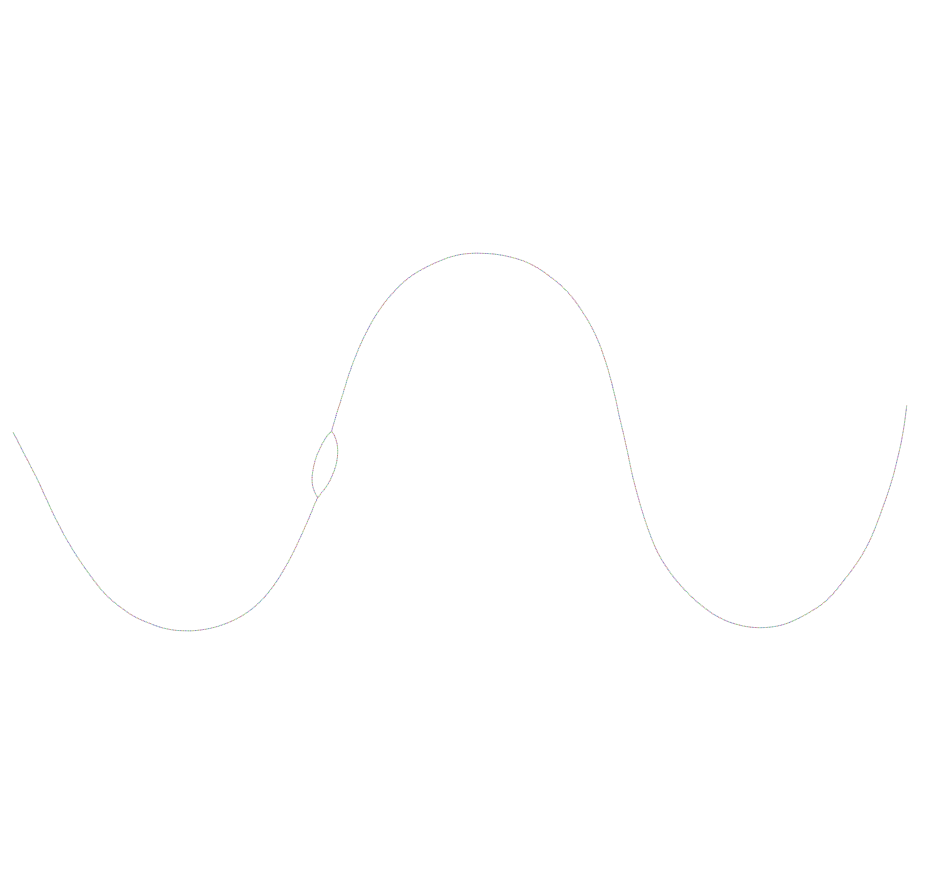
\includegraphics[width=0.5\textwidth]{../toy_dataset/reads_b_k_40.png}
    \caption{Bandage visualization of DBG for k=40}
\end{figure} 

\subsection{Task 1.3.2}

\begin{figure}[h]
    \centering
    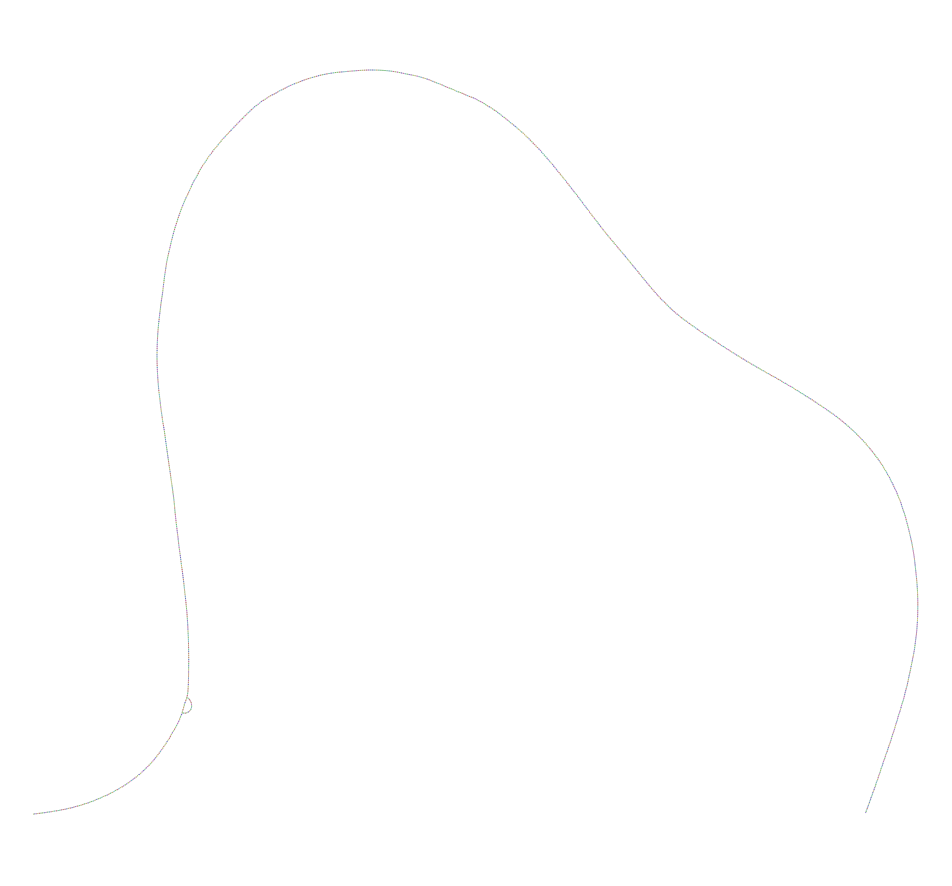
\includegraphics[width=0.5\textwidth]{../toy_dataset/r-k-35.png}
    \caption{Bandage visualization of DBG contigs for k=35 on reads\_r.fastq}
\end{figure} 

\begin{figure}[h]
    \centering
    
\includegraphics[width=0.5\textwidth]{../toy_dataset/r-k-45.png}
    \caption{Bandage visualization of DBG contigs for k=45 on reads\_r.fastq}
\end{figure} 

QUAST evaluation for k=35 and k=45 against reference\_r.fasta:

\begin{center}
\begin{tabular}{ |c|c|c| }
    \hline
    Metric & k=35 & k=45 \\
    \hline
    sequence length & 914 & 1040 \\
    number of contigs & 4 & 1 \\
    GC content (\%) & 51.64 & 51.25 \\
    genome fraction (\%) & 87.885 & 100.000 \\
    duplication ratio & 1.000 & 1.000 \\
    largest contig & 914 & 1040 \\
    N50 & 914 & 1040 \\
    N90 & 914 & 1040 \\
    L50 & 1 & 1 \\
    misassemblies & 0 & 0 \\
    mismatches per 100 kbp & 0.00 & 0.00 \\
    indels per 100 kbp & 0.00 & 0.00 \\
    \hline
\end{tabular}
\end{center}


\subsection{Task 1.3.3}

\subsubsection{ONT reads}
DBG (no-errors) k = 40. OLC (no-errors) m = 40.
DBG (errors) k = 40. OLC (errors) m = 40.
\begin{center}
\begin{tabular}{ |c|c|c||c|c| }
    \hline
    Metric               & DBG (no-errors) & \hl{OLC (no-errors)} & DBG (errors) & \hl{OLC (errors)} \\
    \hline
    sequence length      & 29748  & 1492567  & 76608 & 1505783 \\
    number of contigs    & 1      & 165      & 11 & 163 \\
    GC content (\%)      & 41.27  & 40.68    & 41.21 & 40.84 \\
    genome fraction (\%) & 98.765 & 10000    & 98.738 & 98.655 \\
    duplication ratio    & 1.000  & 50.174   & 1.973 & 37.597 \\
    largest contig       & 29748  & 12465    & 17192 & 20439 \\
    N50                  & 29748  & 9084     & 12088 & 9201 \\
    N90                  & 29748  & 12059    & 1713 & 7834 \\
    L50                  & 1      & 75       & 3 & 73 \\
    misassemblies        & 0      & 0        & 0 & 0 \\
    mismatches per 100 kbp & 0.00 & 0.00     & 78.39 & 493.40 \\
    indels per 100 kbp   & 3.36   & 0.00     & 184.04 & 1463.10  \\
    \hline
\end{tabular}
\end{center}

\subsubsection{HiSeq reads}
DBG (no-errors) k = 40. OLC (no-errors) m = 40.
DBG (errors) k = 40. OLC (errors) m = ??.

\begin{center}
\begin{tabular}{ |c|c|c||c|c| }
    \hline
    Metric & DBG (no-errors) & OLC (no-errors) & DBG (errors) & \hl{OLC (errors)} \\
    \hline
    sequence length        & 29553  & 29553  & 28835 & 10000 \\
    number of contigs      & 3      & 3      & 11 & 10000 \\
    GC content (\%)        & 41.26  & 41.27  & 41.20 & 10000 \\
    genome fraction (\%)   & 97.882 & 97.885 & 94.425 & 10000 \\
    duplication ratio      & 1.002  & 1.002  & 1.014 & 10000 \\
    largest contig         & 12290  & 12290  & 5155 & 10000 \\
    N50                    & 8725   & 8725   & 4682 & 10000 \\
    N90                    & 8538   & 8538   & 1684 & 10000 \\
    L50                    & 2      & 2      & 3 & 10000 \\
    misassemblies          & 0      & 0 & 0  & 0 \\
    mismatches per 100 kbp & 0.00   & 0.00   & 38.16 & 0.00 \\
    indels per 100 kbp     & 10.15  & 0.00   & 38.16 & 0.00 \\
    \hline
\end{tabular}
\end{center}

\subsection{Task 1.3.4}

SPAdes results:

\begin{center}
\begin{tabular}{ |c|c|c|c|c| }
    \hline
    Metric & ONT (no-errors) & ONT (errors) & HiSeq (no-errors) & HiSeq (errors) \\
    \hline
    sequence length & 29748 & 29751 & 29482 & 29482 \\
    number of contigs & 1 & 1 & 1 & 1 \\
    GC content (\%) & 41.27 & 41.25 & 41.26 & 41.26  \\
    genome fraction (\%) & 98.768 & 98.738 & 97.885  & 97.885 \\
    duplication ratio & 1.000 & 1.000 & 1.000 & 1.00 \\
    largest contig & 29748 & 29751 & 29482 & 29482 \\
    N50 & 29748 & 29751 & 29482 & 29482 \\
    N90 & 29748 & 29751 & 29482 & 29482 \\
    L50 & 1 & 1 & 1 & 1 \\
    misassemblies & 0 & 0 & 0 & 0 \\
    mismatches per 100 kbp & 0.00 & 0.00 & 0.00 & 0.00 \\
    indels per 100 kbp & 0.00 & 0.00 & 0.00 & 0.00 \\
    \hline
\end{tabular}
\end{center}
\end{document}
